\newpage
\subsection{Clasificación de imágenes naturales}

	Para poder comprender de mejor manera la sección \ref{subsection: wang_recon_caracteres}, es necesario adentrarse en las particularidades que caracterízan a las imágenes naturales. Dado que, como se ha detallado anteriormente, no es sencillo trabajar con este tipo de imágenes, la siguiente sub-sección se enfoca en las características de las escenas naturales. Las siguientes sub-secciones van a explicar conceptos como el de gradiente que es necesario para poder entender a los descriptores HOG (ver \ref{subsection:hog}) usados tanto por Wang et. al. en \cite{wang}, como por el presente trabajo. Finalmente, se explica el proceso de binarización de los descriptores HOG, necesario para poder usar el clasificador \textit{Random Ferns}.

	\subsubsection{Características}

Las características en las imágenes naturales son muy variadas. Dentro de las mismas podemos encontrar las variaciones de intensidad en la iluminación, la resolución, el ángulo en el que son tomadas, el fondo, las texturas, entre otros. Mas específicamente, dependiendo del objeto que se esté analizando, por ejemplo, texto, surgen más características como el tipo de fuente, el tamaño, la posición y orientación de los caracteres, la contaminación que pueda llegar a tener el texto por suciedad u oclusión, etc. La infita variedad que es posible encontrar en este tipo de imágenes, dificultan el trabajo de reconocimiento sobre ellas por lo que, en general, es necesario realizar un pre-procesamiento antes de usarlas.

	En el caso del reconocimiento de texto, dada la gran cantidad de formas en que se puede encontrar la imagen de un carácter, es necesario encontrar algún método que extraiga las características mas representativas para poder distinguilo. Para poder analizar los caracteres en las imágenes naturales, uno de los enfoques que adoptan Wang et al. en \cite{wang} es el de trabajar con el descriptor HOG de cada imagen. Para poder entender que es un descriptor HOG (que se detalla en \ref{subsection:hog}), primero es necesario comprender el concepto de gradiente que se explica a continuación.
	
	%\paragraph{Imágenes naturales} ~\\

	\textbf{Cambiar el título}
	
	Las imágenes naturales siempre han sido un tema de interés en el campo de investigación de visión por computadora. La cantidad de información que puede proveer una imagen es gigantesca y la necesidad de poder procesar y reconocer es información ha llevado a los investigadores a proponer métodos para poder procesarla.	Aparte del puro interés científico, la popularidad se debe a la cantidad de aplicaciones prácticas que tiene el tema. Uno de los ejemplos más claros es el reconocimiento de patentes o LPR(por sus siglas en inglés)~\cite{DAB}, o el reconomiento de personas~\cite{DT05}, entre otros; sin embargo, no es una tarea sencilla ya que las imágenes naturales tienen infinitas variaciones que hacen díficil el reconomiento de objetos dentro de ellas.
	
	
	\subparagraph{Características} ~\\
	
		Las características en las imágenes naturales son muy variadas. Todas estas variaciones dificultan el trabajo sobre ellas por lo cual en general es necesario realizar un trabajo de pre-procesamiento antes de trabajar con las mismas. Las características que podemos encontrar en este tipo de imágenes son las variaciones de intensidad en la iluminación, la resolución, el ángulo en el que son tomadas las mismas, el fondo, las texturas, entre otros. Mas específicamente, dependiendo del objeto que se esté analizando, por ejemplo, texto en imágenes naturales, surgen más características como el tipo de fuente, el tamaño, la posición y orientación de los caracteres en el texto, la contaminación que pueda llegar a tener el texto por suciedad u oclusión, etc.
	
\paragraph{Gradientes} ~\\

	Sea $f(x_1,\dots,x_n)$ una función escalar de múltiples variables. El gradiente de $f$ representa la pendiente de la tangente del gráfico de $f$.  Mas precisamente, el gradiente apunta en la dirección donde se registra la mayor tasa de incremento de la función $f$ y su magnitud es la pendiente del gráfico de $f$ en esa dirección. Formalmente, es la generalización del concepto de derivada en funciones de múltiples variables.
		
	El gradiente de la función $f$ descripta anteriormente, es denotado como $\nabla f$ donde $\nabla$(el símbolo nabla) denota el operador diferencial. El gradiente de $f$ es definido como el único campo vectorial cuyo producto punto con cualquier vector $v$ en cada punto $x$ es la derivada direccional de $f$ a lo largo de $v$. Es decir,
		 \begin{align*}
		 	(\nabla f(x))\cdot v = D_v f(x)
		 \end{align*}
		 
	En un sistema de coordenadas rectangular, el gradiente es el campo vectorial cuyos componentes son las derivadas parciales de $f$:
		 
		 \begin{align*}
		 	\nabla f(x) = \frac{\partial f}{\partial x_1}\mathbf{e}_1 + \cdots + \frac{\partial f}{\partial x_n }\mathbf{e}_n
		 \end{align*}
	donde los $\mathbf{e}_i$ son vectores unitarios ortogonales que apuntan en la dirección de coordenadas.

	En el procesamiento de imágenes, un gradiente es un cambio direccional en la intensidad o color de la imagen. El vector gradiente se forma combinando la derivada parcial de la imagen en las direcciones $x$ e $y$. Se puede expresar del a siguiente forma:
		\begin{align}
			\nabla I = \left( \frac{\partial I}{\partial x} , \frac{\partial I}{\partial y} \right)
		\end{align}	
		
	Cuando determinamos la derivada parcial de $I$ respecto de $x$, determinamos la rapidez con que la imagen cambia de intensidad a medida que $x$ cambia. Para funciones continuas, $I(x,y)$, podemos expresarlo de la siguiente manera:
	\begin{align}
		\frac{\partial I(x,y)}{\partial x} = \lim_{\nabla x\rightarrow 0} \frac{I(x + \nabla x, y) - I(x,y)}{\nabla x}	
	\end{align}
	
	 El calculo de los gradientes de una imagen es útil ya que sirve, por ejemplo, para realizar detección de bordes de un objeto. En este caso, después de que los gradientes han sido computados, los píxeles con alto valor de gradiente son elegido como posibles bordes. Los píxeles con el valor de gradiente más alto en la dirección del gradiente se convierten en píxeles de borde. Los gradientes, también pueden ser usados en aplicaciones que realizan reconocimiento de objetos o correspondencia de texturas \textbf{agregar referencias}.

	
\subsubsection{Gradientes}
\label{subsubsection: Gradientes}

Sea $f(x_1,\dots,x_n)$ una función escalar de múltiples variables. Como expresa Gonzales et. al. en \cite{GonWoods}, el gradiente de $f$ es un vector que apunta en la dirección donde se registra la mayor tasa de incremento de la función. Su magnitud es la pendiente del gráfico en esa dirección. Es la generalización del concepto de derivada en funciones de múltiples variables.
		
	El gradiente de la función $f$ descrita anteriormente, es denotado como $\nabla f$ donde $\nabla$ (el símbolo nabla) denota el operador diferencial. El gradiente de $f$ es definido como el único campo vectorial cuyo producto punto con cualquier vector $v$ en cada punto $x$ es la derivada direccional de $f$ a lo largo de $v$. Es decir,
		 \begin{align*}
		 	(\nabla f(x))\cdot v = D_v f(x)
		 \end{align*}
		 
	En un sistema de coordenadas rectangular, el gradiente es el campo vectorial cuyos componentes son las derivadas parciales de $f$:
		 
		 \begin{align*}
		 	\nabla f(x) = \frac{\partial f}{\partial x_1}\mathbf{e}_1 + \cdots + \frac{\partial f}{\partial x_n }\mathbf{e}_n
		 \end{align*}
	donde los $\mathbf{e}_i$ son vectores unitarios ortogonales que apuntan en la dirección de coordenadas.

	En el procesamiento de imágenes, un gradiente es un cambio direccional en la intensidad o color de la imagen. En \cite{DJacobs}, Jacobs explica que el vector gradiente se forma combinando la derivada parcial de la imagen en las direcciones $x$ e $y$. Se puede expresar del a siguiente forma:
		\begin{align}
			\nabla I = \left( \frac{\partial I}{\partial x} , \frac{\partial I}{\partial y} \right)
		\end{align}	
		
	donde \textit{I}: $\mathbb{R}^{2} \rightarrow [0, 1]$ es la ``función intensidad'' que asigna un valor de intensidad a cada pixel (par (x,y)) de la imagen. Según Jacobs, cuando determinamos la derivada parcial de $I$ respecto de $x$, determinamos la rapidez con que la imagen cambia de intensidad a medida que $x$ cambia. Para funciones continuas, $I(x,y)$, podemos expresarlo de la siguiente manera:
	\begin{align}
		\frac{\partial I(x,y)}{\partial x} = \lim_{\nabla x\rightarrow 0} \frac{I(x + \nabla x, y) - I(x,y)}{\nabla x}	
	\end{align}
	
	 El cálculo de los gradientes de una imagen es útil ya que sirve, por ejemplo, para realizar detección de bordes de un objeto. La detección de bordes busca identificar puntos en una imagen en donde el brillo de la misma cambie de manera abrupta o, más formalmente, tenga discontinuidades. El propósito de esto es capturar eventos importantes o cambios en las propiedades de una imagen. En este caso, después de que los gradientes han sido computados, los píxeles con alto valor de gradiente son elegido como posibles bordes. Los píxeles con el valor de gradiente más alto en la dirección del gradiente se convierten en píxeles de borde. Los gradientes, también pueden ser usados en aplicaciones que realizan reconocimiento de objetos o correspondencia de texturas.	 
	
	\subsubsection{Características locales}

		\paragraph{Descriptor SIFT} ~\\

	\textit{Scale-invariant feature transform} o SIFT (por su sigla en inglés) es un algoritmo en visión por computadora desarrollado por David G. Lowe \cite{LoweDavid04} para detectar y describir las características locales de una imagen. Estas características, como se explico en secciones anteriores, sirven para identificar a una clase de interés u objeto cuando se la trata de localizar dentro de una imagen donde hay varios objetos. Los descriptores SIFT tienen la característica de no alterarse ante un cambio en la escala o en la orientación y son robustos en el sentido de que pueden detectar objetos si estos están desordenados o si los mismos están parcialmente ocultos. Además, son parcialmente invariantes a las transformaciones afines y a los cambios en la iluminación.
		
	Para obtener estas características, se realiza un muestreo de las orientaciones y magnitudes del gradiente de la imagen. En el trabajo de Lowe, este muestreo se realiza sobre regiones de $16 \times 16$ alrededor del punto de interés. Se analizan las muestras de cada región de $16 \times 16$ formando histogramas de orientaciones resumiendo el contenido en sub-regiones de $4 \times 4$. Cada uno de los histogramas se compone de 8 orientaciones. Por lo tanto se obtienen 16 histogramas respecto de las orientaciones de los puntos de cada región para cada uno de los puntos de interés. Finalmente el descriptor de cada punto de interés está formado por un vector que contiene los valores de las 8 orientaciones de los $4 \times 4$ histogramas, con lo cual se obtendría un vector de 128 elementos.

	Dado que los cambios en la iluminación afectan en mayor medida a la magnitud del gradiente y no a la orientación, se busca una representación de esta magnitud que minimice estos efectos. El objetivo es modificar al vector para darle cierta robustez frente a cambios en la iluminación. Para eso se lleva a cabo un proceso de normalización, donde los cambios en la luminosidad no afecta a los valores del gradiente. Finalmente, se limita el valor de cada componente de magnitud de gradiente a un valir máximo para que tenga un mayor peso la orientación frente a la magnitud del gradiente. Siguiendo los parámetros de Lowe en \cite{LoweDavid04}, el valor del umbral es de 0,2. Luego se vuelve a normalizar a una amplitud de unidad.

	
		
	
		\paragraph{Histograma de gradientes orientados} ~\\
\label{subsection:hog}

	Histograma de Gradientes Orientados o HOG (por sus siglas en inglés), son descriptores de características utilizados en visión por computadora y en el procesamiento de imágenes con el objetivo de realizar detección de objetos. Fueron introducidos por N. Dalal y B. Triggs en~\cite{DT05} con el propósito de realizar detección de personas; sin embargo, su uso no se limita solamente a esa área, sino que pueden ser utilizados en otras áreas como la detección de caracteres tal y como hizo Wang et al. en \cite{wang}.
	
	Todas las imágenes, como por ejemplo la presentada en la figura~\ref{fig: Imagen Letra original}, contienen objetos locales cuyas apariencias y formas pueden ser descriptas por la distribución de los gradientes de intensidad como se puede observar en la figura~\ref{fig: Image HOG}.	Un descriptor HOG, es un vector compuesto por una combinación de histogramas que representan los gradientes de intesidad en distintas regiones de una imagen. La implementación de estos descriptores, se obtiene dividiendo a la imagen en regiones de tamaño fijo llamadas celdas como se puede observar en la figura~\ref{fig: Image HOG celdas} y posteriormente, por cada celda, se calcula un histograma de gradientes para los píxeles en la celda ~\ref{fig: Cell Histogram}. Finalmente, como se explico anteriormente, el descriptor se obtiene de combinar los histogramas obtenidos~\ref{fig: Vector HOG}. La precisión se puede incrementar si se normalizan los histogramas, es decir, si se calcula una medida de la intensidad en una región más grande de la imagen, denominada bloque y se utiliza dicho valor para normalizar las celdas contenidas en el bloque.
	
	%El descriptor HOG mantiene una cuantas ventajas con respecto a otros métodos descriptores. Dado que el descriptor HOG opera en celdas localizadas, el método mantiene la invarianza a transformaciones geométricas y fotométricas, excepto para la orientación de objetos. Dichos cambios sólo aparecerían en regiones espaciales grandes~\cite{DT05}.
	
	En el área de visión por computadora, los descriptores HOG son considerados estado del arte o \textit{state of the art} al igual que muchos otros descriptores como \textit{SIFT}, \textit{Geometric Blur}, \textit{Shape Context}, \textit{Patch descriptor}, \textit{Maximum Response of filters} y \textit{Spin image}. Los descriptores HOG, han demostrado ser útiles en la clasificación como se puede apreciar en el trabajo de Wang et al.~\cite{wang} donde se ha entrenado el clasificador Random Ferns con estos. Incluso, se puede decir que la performance obtenida con estos descriptores en dicho trabajo supera a la mayoría de los descriptores evaluados en el trabajo de De Campos et al.~\cite{dCBV09} bajo las mismas condiciones de entrenamiento. Si bien Wang et al. usan como clasificador a Random Ferns y De Campos et al. usan en su evaluación SVM, se puede apreciar en la clasificación el impacto positivo al utilizar los descriptores HOG.
	
	La binarización de los descriptores HOG es necesaria, ya que las características binarias son fáciles de computar, son compactas, se pueden almacenar fácilmente y son fáciles de comparar. En cambio, los descriptores originales tienen alta dimensionalidad y requieren sistemas con más memoria, capacidad de almacenamiento y procesamiento. Uno de los beneficios de este enfoque en la clasificación, es que escala bien con la cantidad de categorías o clases. Muchos sistemas en tiempo real como el reconocimiento de objetos~\cite{SJC08} y en el agrupamiento de puntos clave~\cite{OFL07} han incorporado este enfoque por su utilidad.

	
	\paragraph{Binarización} ~\\

		A continuación se explicará un método para la binarización de los descriptores HOG. Para binarizar es necesario calcular un vector umbral. El umbral se calcula de la siguiente manera:
		\begin{itemize}
			\item Dado $N$ descriptores HOG de dimension $D$, se forma una matriz de tamaño $N \times D$ donde cada fila representa un vector.
			\item Se seleccionan $X$ columnas al azar de la matriz con reemplazo.
			\item Respetando el orden en que fueron seleccionadas, se aplica una función sobre cada columna (la función puede ser el calculo de la mediana, la media, bootstrap, entre otros), obteniendo de esta manera un vector nuevo $W$ de dimensión $X$ tal que cada dimensión de $W$ está compuesta por un par $(z,y)$ donde $y$ es un número talque $0 \leq y \leq D$ que representa una de las columnas elegidas de la matriz y $z$ representa el valor resultante de haber aplicado la función elegida a dicha columna. Cabe aclarar que $X$ puede ser mayor o menor a $D$ por lo cual el umbral $W$ puede tener mayor o menor dimensión al final.
		\end{itemize}
		Posteriormente dicho umbral $W$ se utiliza para binarizar los vectores originales de manera sencilla: sea $v_j$ con $j \in \{1,\dots,N\}$ uno de los $N$ vectores originales y tal que $v_j = d_1,d_2,\dots,d_D$. Luego se compara cada dimensión del umbral $W$ con la $y$-esima dimensión del vector $v_j$. Si $d_y \leq z$ se asigna 0, caso contrario 1. De esta manera binarizamos el vector $v_j$ obteniendo un nuevo vector binario de dimensión $X$.

		\begin{figure}[htbp]
			\centering
			\subfloat[Imagen original\label{fig: Imagen Letra original}]{
				\fbox{ 
\includegraphics[scale=0.3]{img/letter_A.jpg} }
			}
			\subfloat[Descriptores HOG de la imagen original\label{fig: Image HOG}]{
				\fbox{ 
\includegraphics[scale=0.3]{img/letter_A_HOG.jpg} }
			}
			\\
			\subfloat[División por bloques de tamaño 4x4 celdas\label{fig: Image HOG celdas}]{
				\fbox{ 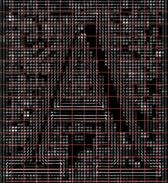
\includegraphics[scale=0.6]{img/letter_A_with_cells_2.jpg} }
			}
			\subfloat[Histograma de una celda\label{fig: Cell Histogram}]{
				\fbox{ 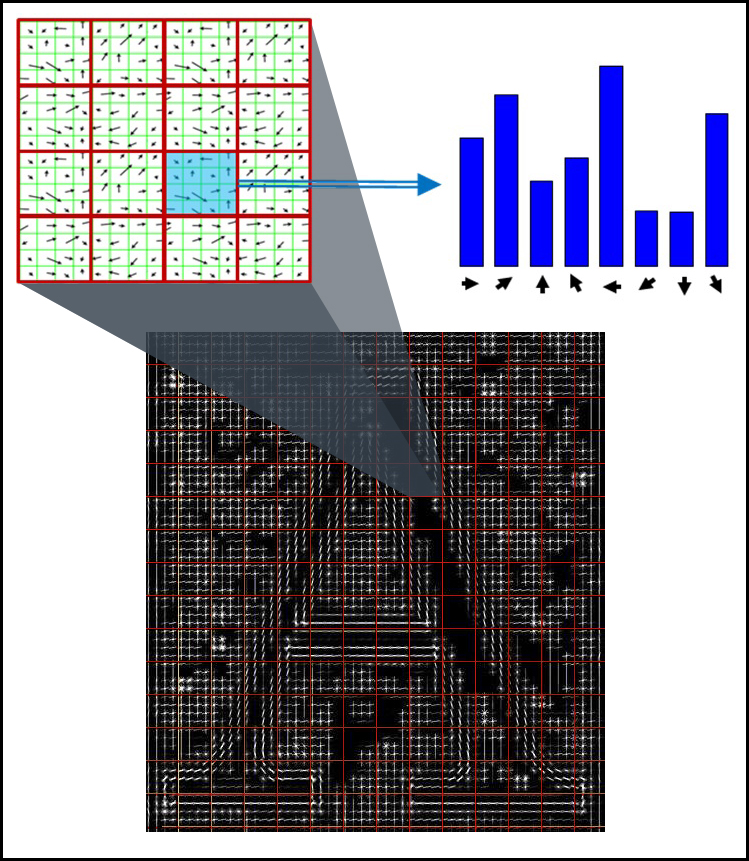
\includegraphics[scale=1.5]{img/letter_A_histogram.jpg} }
			}
			\caption{Descriptores HOG de la imagen de un caracter}
			\label{fig: HOG features}
		\end{figure}	

		\begin{figure}[htbp]
			\centering
			\fbox{ 
\includegraphics[scale=1]{img/feature_vector.jpg} }
			\caption[Vector HOG]{Formación del vector de características a partir de la concatenación de los histogramas. \textbf{CAMBIAR IMAGEN por algo mejor}}
			\label{fig: Vector HOG}
		\end{figure}

	
	%\subsubsection{Reconocimiento de objetos}
